\documentclass[]{article}
\usepackage{geometry}
\geometry{legalpaper, margin=1.2in}
\usepackage[protrusion=true,expansion=true]{microtype}	
\usepackage[boxruled,linesnumbered,vlined,inoutnumbered]{algorithm2e}
\SetKwInOut{Parameter}{Parameters}
\usepackage{amsmath}
\usepackage{amsthm}
\usepackage{amssymb}
\usepackage{mathtools}
\usepackage{mathrsfs}
\usepackage{soul}
\usepackage{natbib}
\usepackage{rotating}
\usepackage{gensymb}
\usepackage{lscape}
\usepackage{array}
\usepackage{makecell}
\renewcommand\theadalign{bc}
\renewcommand\theadfont{\bfseries}
\renewcommand\theadgape{\Gape[4pt]}
\renewcommand\cellgape{\Gape[4pt]}
\usepackage{courier}
\usepackage{lipsum}
\usepackage{graphicx}
\usepackage{subcaption}
\usepackage[space]{grffile}
\usepackage{xcolor}
\definecolor{light-grey}{rgb}{0.9,0.9,0.9}
\definecolor{dark-red}{rgb}{0.4,0.15,0.15}
\definecolor{dark-blue}{rgb}{0,0,0.7}
\usepackage{environ}
\setcounter{tocdepth}{2}
\renewcommand{\contentsname}{Table of Contents}
\usepackage{hyperref}
\hypersetup{
    colorlinks, linkcolor={dark-blue},
    citecolor={dark-blue}, urlcolor={dark-blue}
}
\newcommand{\HIGHLIGHT}[1]{\textcolor{blue}{\textbf{#1}}}
\newcommand{\TODO}[1]{\textcolor{red}{\textbf{#1}}}

\begin{document}




%-----------------
%	Homework 1
%-----------------
\newpage
\begin{center}
    \begin{Large}
    COMPSCI 589 Homework 1 - Spring 2022
    \end{Large}
    \\
    \HIGHLIGHT{Due February 15, 2022, 11:55pm Eastern Time}
\end{center}
\addcontentsline{toc}{subsection}{\textbf{Homework 1}}



\vspace{0.25in}
\section{Instructions}

\begin{itemize}
    \item This homework assignment consists of a programming portion. While you may discuss problems with your peers, you must answer the questions on your own and implement all solutions independently. In your submission, do explicitly list all students with whom you discussed this assignment. 
    \item We strongly recommend that you use \LaTeX~to prepare your submission. The assignment should be submitted on Gradescope as a PDF with marked answers via the Gradescope interface. The source code should be submitted via the Gradescope programming assignment as a .zip file. Include with your source code instructions for how to run your code. 
    \item We strongly encourage you to use Python 3 for your homework code. You may use other languages. In either case, you \textit{must} provide us with clear instructions on how to run your code and reproduce your experiments. 
    \item You may \textit{not} use any machine learning-specific libraries in your code, e.g., TensorFlow, PyTorch, or any machine learning algorithms implemented in scikit-learn (though you may use other functions provided by this library, such as one that splits a dataset into training and testing sets). You may use libraries like numpy and matplotlib. If you are not certain whether a specific library is allowed, do ask us.
    \item All submissions will be checked for plagiarism using two independent plagiarism-detection tools. Renaming variable or function names, moving code within a file, etc., are all strategies that \textit{do not} fool the plagiarism-detection tools we use. \textcolor{red}{If you get caught, all penalties mentioned in the syllabus \textit{will} be applied---which may include directly failing the course with a letter grade of ``F''}.
    \item The tex file for this homework (which you can use if you decide to write your solution in \LaTeX) can be found \href{https://people.cs.umass.edu/~bsilva/courses/CMPSCI_589/Spring2022/homeworks/hw1.zip}{here}.
    \item The automated system will not accept assignments after \HIGHLIGHT{11:55pm on February 15}. 
\end{itemize}

\newpage

\vspace{1cm}
\section*{Programming Section (100 Points Total)}

In this section of the homework, you will implement two classification algorithms: \textit{k}-NN and Decision Trees. \textbf{Notice that you may \ul{not} use existing machine learning code for this problem: you must implement the learning algorithms entirely on your own and from scratch.} 

\vspace{0.35in}

\begin{enumerate}
    \item {\LARGE{\textbf{Evaluating the \textit{k}-NN Algorithm}}}\\\HIGHLIGHT{(50 Points Total)}\\
    \vspace{0.1in}
    
    In this question, you will implement the \textit{k}-NN algorithm and evaluate it on a standard benchmark dataset: the Iris dataset. Each instance in this dataset contains (as attributes) four properties of a particular plant/flower. The goal is to train a classifier capable of predicting the flower's species based on its four properties. \textbf{You can download the dataset \href{https://people.cs.umass.edu/~bsilva/courses/CMPSCI_589/Spring2022/homeworks/datasets/iris.csv}{here}.}
    
    The Iris dataset contains 150 instances. Each instance is stored in a row of the CSV file and is composed of 4 attributes of a flower, as well as the species of that flower (its label/class). The goal is to predict a flower's species based on its 4 attributes. More concretely, each training instance contains information about the length and width (in centimeters) of the \href{https://en.wikipedia.org/wiki/Sepal}{sepal} of a flower, as well as the length and width (in centimeters) of the flower's \href{https://en.wikipedia.org/wiki/Petal}{petal}. The label associated with each instance indicates the species of that flower: Iris Versicolor, Iris Setosa, or Iris Virginica. See Figure~\ref{fig:iris} for an example of what these three species of the Iris flower look like.
    %
    In the CSV file, the attributes of each instance are stored in the first 4 columns of each row, and the corresponding class/label is stored in the last column of that row.
    
    \begin{figure}[h!!!]
        \centering
        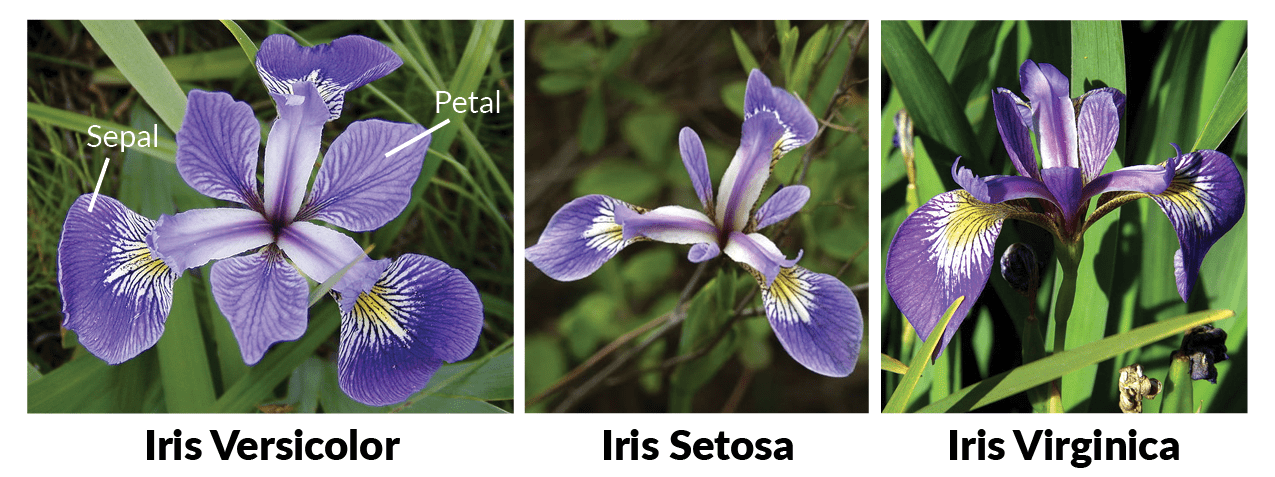
\includegraphics[width=0.75\textwidth]{figures/iris-picture.png}
        \caption{Pictures of three species of the Iris flower (Source: \href{https://www.datacamp.com/community/tutorials/machine-learning-in-r}{Machine Learning in R for beginners}).}
        \label{fig:iris}
    \end{figure}
    
    The goal of this experiment is to evaluate the impact of the parameter \textit{k} on the algorithm's performance when used to classify instances in the training data, and also when used to classify new instances. For each experiment described below, you should use Euclidean distance as the distance metric and then follow these steps:
    
    \begin{enumerate}
        \item shuffle the dataset to make sure that the order in which examples appear in the dataset file does not affect the learning process;\footnote{If you are writing Python code, you can shuffle the dataset by using, e.g., the \texttt{sklearn.utils.shuffle} function.}
        %
        \item randomly partition the dataset into disjoint two subsets: a \textit{training set}, containing 80\% of the instances selected at random; and a testing set, containing the other 20\% of the instances. Notice that these sets should be disjoint: if an instance is in the training set, it should not be in the testing set, and vice-versa.\footnote{If you are writing Python code, you can perform this split automatically by using the \texttt{sklearn.model\_selection.train\_test\_split} function.} The goal of splitting the dataset in this way is to allow the model to be trained based on just part of the data, and then to ``pretend'' that the rest of the data (i.e., instances in the testing set, which were \textit{not} used during training) correspond to new examples on which the algorithm will be evaluated. If the algorithm performs well when used to classify examples in the testing set, this is evidence that it is generalizing well the knowledge it acquired after learning based on the training examples;
        %
        \item train the \textit{k}-NN algorithm using \textit{only} the data in the training set;
        %
        \item compute the \textit{accuracy} of the \textit{k}-NN model when used to make predictions for instances in the \textit{training set}. To do this, you should compute the percentage of correct predictions made by the model when applied to the training data; that is, the number of correct predictions divided by the number of instances in the training set;
        %
        \item compute the \textit{accuracy} of the \textit{k}-NN model when used to make predictions for instances in the \textit{testing set}. To do this, you should compute the percentage of correct predictions made by the model when applied to the testing data; that is, the number of correct predictions divided by the number of instances in the testing set. 
    \end{enumerate}
    
    \textcolor{red}{\textbf{Important: when training a \textit{k}-NN classifier, do not forget to normalize the features!}}
    
    
    \newpage
    You will now construct two graphs. The first one will show the accuracy of the \textit{k}-NN model (for various values of \textit{k}) when evaluated on the training set. The second one will show the accuracy of the \textit{k}-NN model (for various values of \textit{k}) when evaluated on the testing set. You should vary \textit{k} from 1 to 51, using only odd numbers ($1, 3, \ldots, 51$). For each value of \textit{k}, you should run the process described above (i.e., steps \textit{(a)} through \textit{(e)}) 20 times. This will produce, for each value of \textit{k}, 20 estimates of the accuracy of the model over training data, and 20 estimates of the accuracy of the model over testing data. 
    
    \vspace{0.3in}
    
    \HIGHLIGHT{Q1.1 (12 Points)} In the first graph, you should show the value of \textit{k} on the horizontal axis, and on the vertical axis, the average accuracy of models trained over the \textit{training set}, given that particular value of \textit{k}. Also show, for each point in the graph, the corresponding standard deviation; you should do this by adding error bars to each point. The graph should look like the one in Figure~\ref{fig:sample_graph} (though the ``shape'' of the curve you obtain may be different, of course).
    %
    \begin{figure}[ht!]
        \centering
        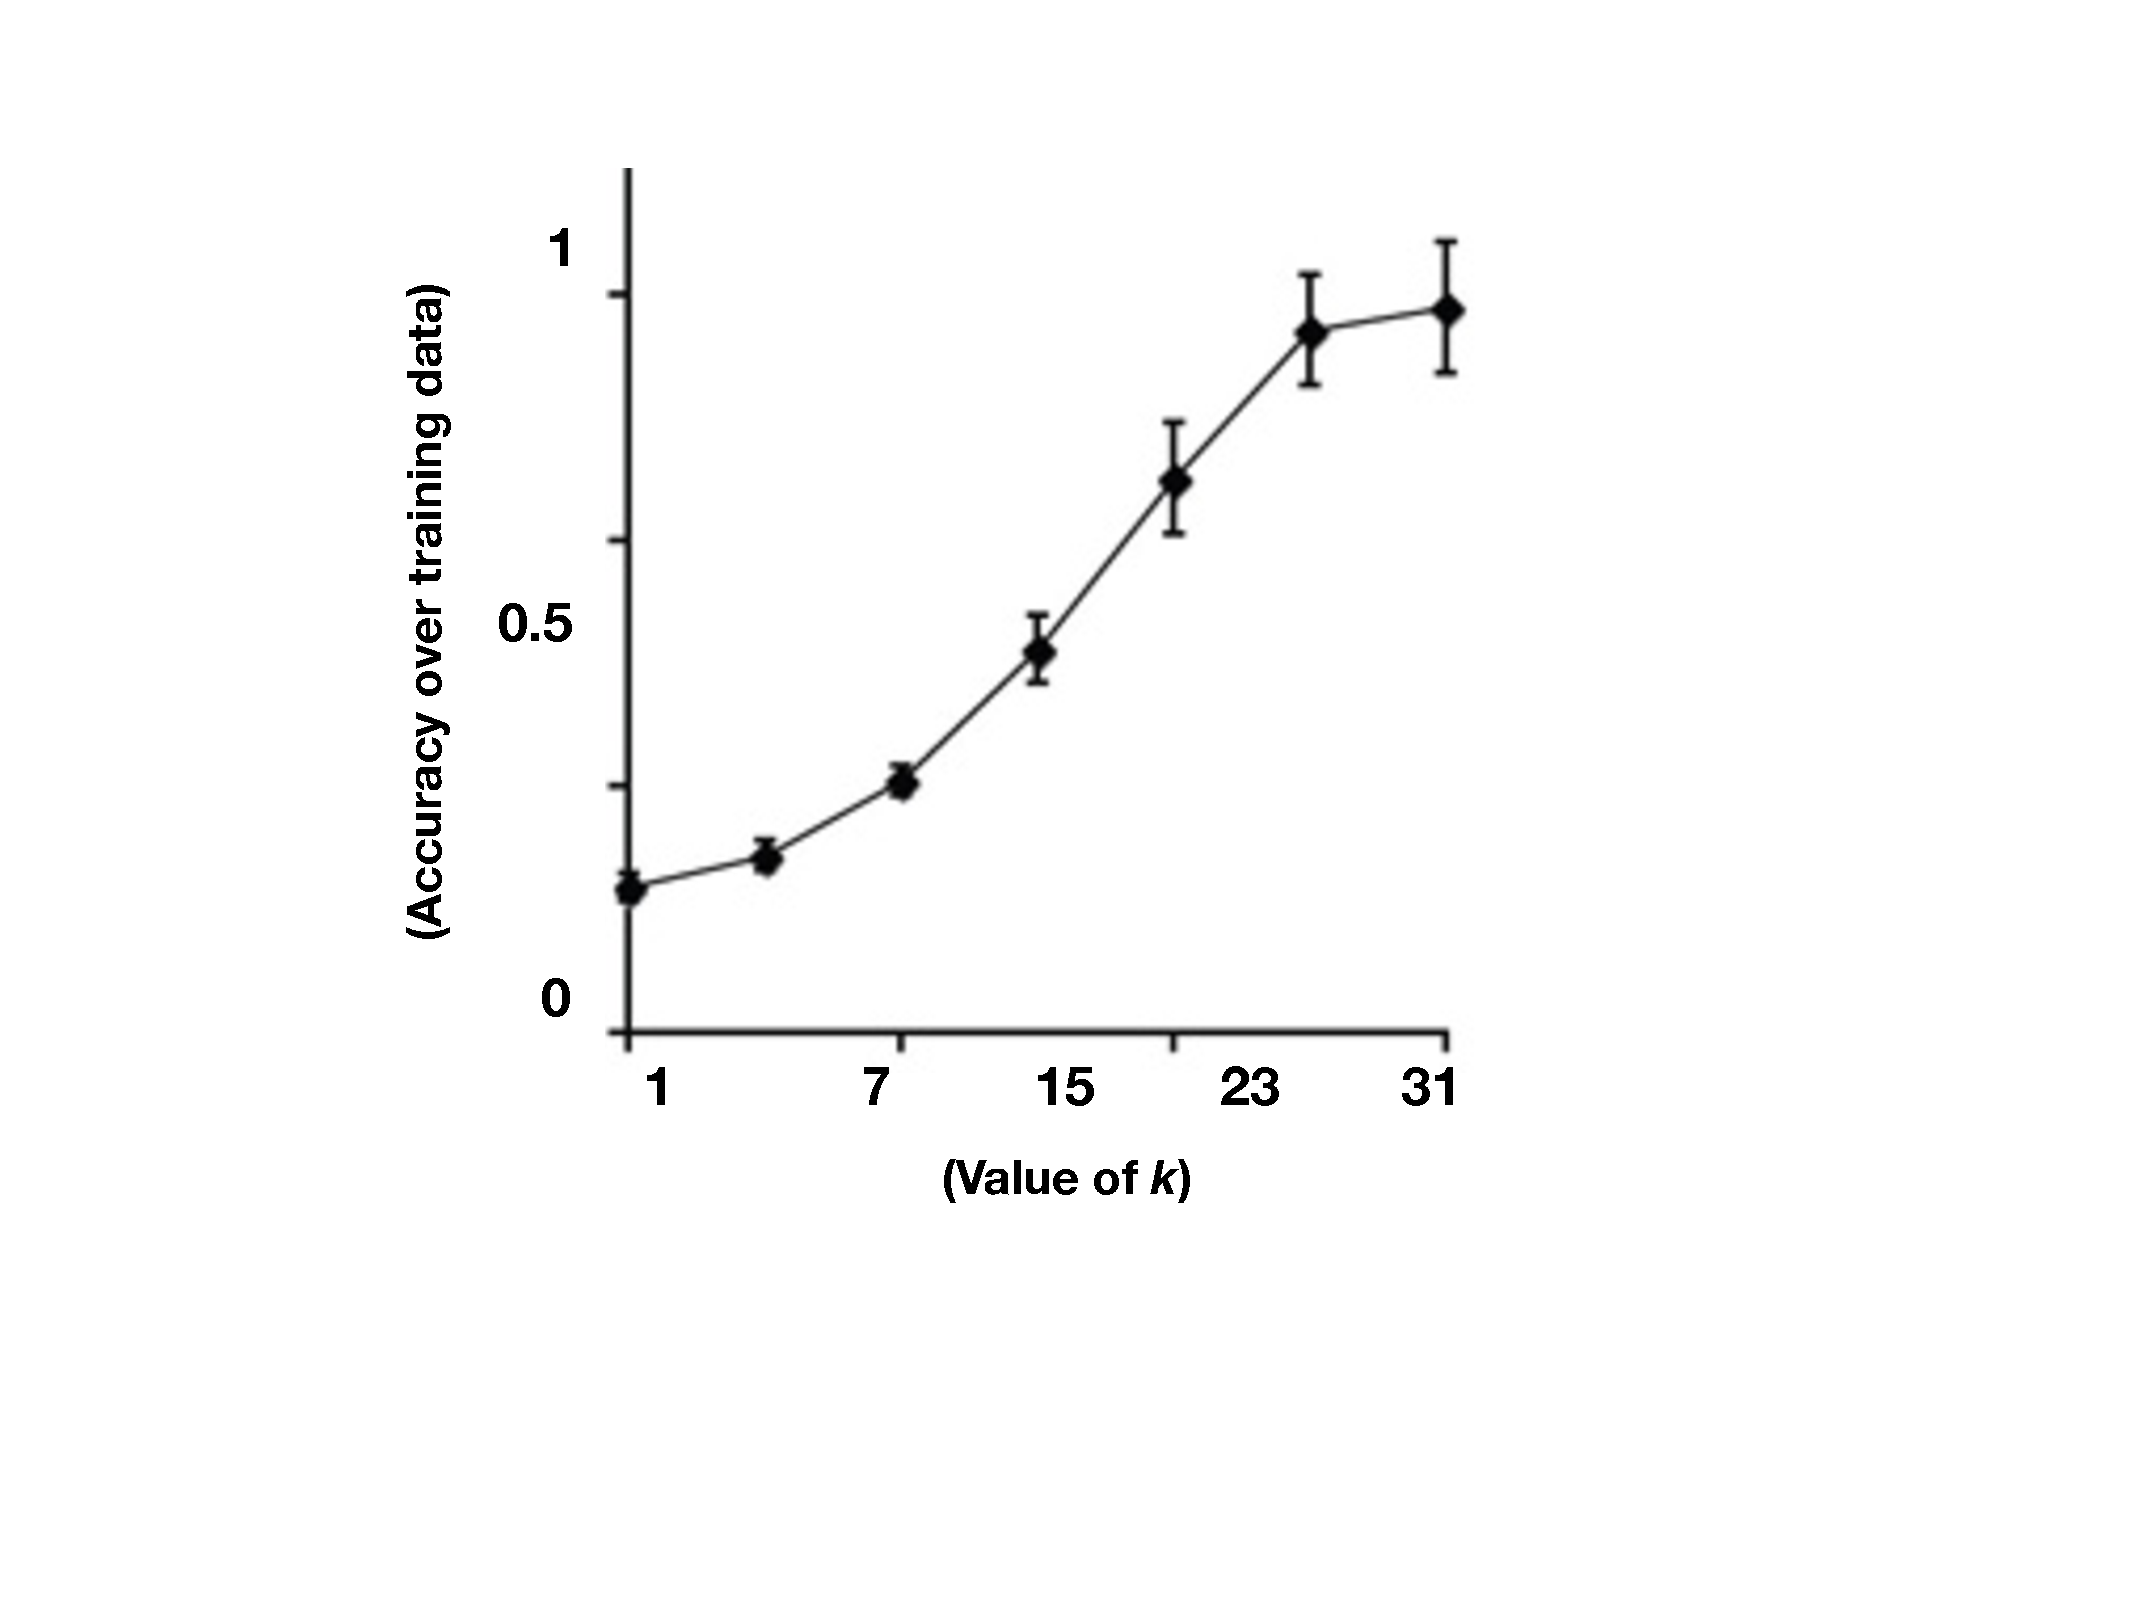
\includegraphics[width=0.4\textwidth]{figures/example_graph.pdf}
        \caption{Example showing how your graphs should look like. The ``shape'' of the curves you obtain may be different, of course.}
        \label{fig:sample_graph}
    \end{figure}   
    %
    % YOUR RESPONSE HERE
    %
    
    
    \HIGHLIGHT{Q1.2 (12 Points)} In the second graph, you should show the value of \textit{k} on the horizontal axis, and on the vertical axis, the average accuracy of models trained over the \textit{testing set}, given that particular value of \textit{k}. Also show, for each point in the graph, the corresponding standard deviation by adding error bars to the point.
    %
    % YOUR RESPONSE HERE
    %


    \HIGHLIGHT{Q1.3 (10 Points)} Explain intuitively why each of these curves look the way they do. First, analyze the graph showing performance on the training set as a function of \textit{k}. Why do you think the graph looks like that? Next, analyze the graph showing performance on the testing set as a function of \textit{k}. Why do you think the graph looks like that?
    %
    % YOUR RESPONSE HERE
    %
    
    
    \HIGHLIGHT{Q1.4 (8 Points)} We say that a model is \textit{underfitting} when it performs poorly on the training data (and most likely on the testing data as well). We say that a model is \textit{overfitting} when it performs well on training data but it does not generalize to new instances. Identify and report the ranges of values of \textit{k} for which \textit{k}-NN is underfitting, and ranges of values of \textit{k} for which \textit{k}-NN is overfitting.
    %
    % YOUR RESPONSE HERE
    %
    
    
    \HIGHLIGHT{Q1.5 (8 Points)} Based on the analyses made in the previous question, which value of \textit{k} you would select if you were trying to fine-tune this algorithm so that it worked as well as possible in real life? Justify your answer.
    %
    % YOUR RESPONSE HERE
    %
    
    
    
    %------------------------------------------------------
    
    
    \vspace{0.5in}
    \item {\LARGE{\textbf{Evaluating the Decision Tree Algorithm}}} \\\HIGHLIGHT{(50 Points Total)}\\
    \vspace{0.1in}

    In this question, you will implement the Decision Tree algorithm, as presented in class, and evaluate it on the \textit{1984 United States Congressional Voting} dataset. This dataset includes votes for each U.S. House of Representatives Congressperson on the 16 key votes. For each topic/law being considered, a congressperson may have voted yea, nay, or may not have voted. Each of the 16 attributes associated with a congressperson, thus, has 3 possible categorical values. The goal is to predict, based on the voting patterns of politicians (i.e., on how they voted on those 16 cases), whether they are a Democrat (class/label 0) or a Republican (class/label 1). \textbf{You can download the dataset \href{https://people.cs.umass.edu/~bsilva/courses/CMPSCI_589/Spring2022/homeworks/datasets/house_votes_84.csv}{here}.}
    
    Notice that this dataset contains 435 instances. Each instance is stored in a row of the CSV file. The first row of the file describes the name of each attribute. The attributes of each instance are stored in the first 16 columns of each row, and the corresponding class/label is stored in the last column of that row. For each experiment below, you should repeat the steps \textit{(a)} through \textit{(e)} described in the previous question. You should use the Information Gain criterion to decide whether an attribute should be used to split a node.

    You will now construct two histograms. The first one will show the accuracy distribution of the Decision Tree algorithm when evaluated on the training set. The second one will show the accuracy distribution of the Decision Tree algorithm when evaluated on the testing set. You should train the algorithm 100 times using the methodology described above (i.e., shuffling the dataset, splitting the dataset into disjoint training and testing sets, computing its accuracy in each one, etc.). This process will result in 100 accuracy measurements for when the algorithm was evaluated over the training data, and 100 accuracy measurements for when the algorithm was evaluated over testing data. 
    
    
    \vspace{0.3in}
    
    \HIGHLIGHT{Q2.1 (12 Points)} In the first histogram, you should show the accuracy distribution when the algorithm was evaluated over \textit{training data}. The horizontal axis should show different accuracy values, and the vertical axis should show the frequency with which that accuracy was observed while conducting these 100 experiments/training processes. The histogram should look like the one in Figure~\ref{fig:sample_histogram} (though the ``shape'' of the histogram you obtain may be different, of course). You should also report the mean accuracy and its standard deviation.
    %
    \begin{figure}[ht!]
        \centering
        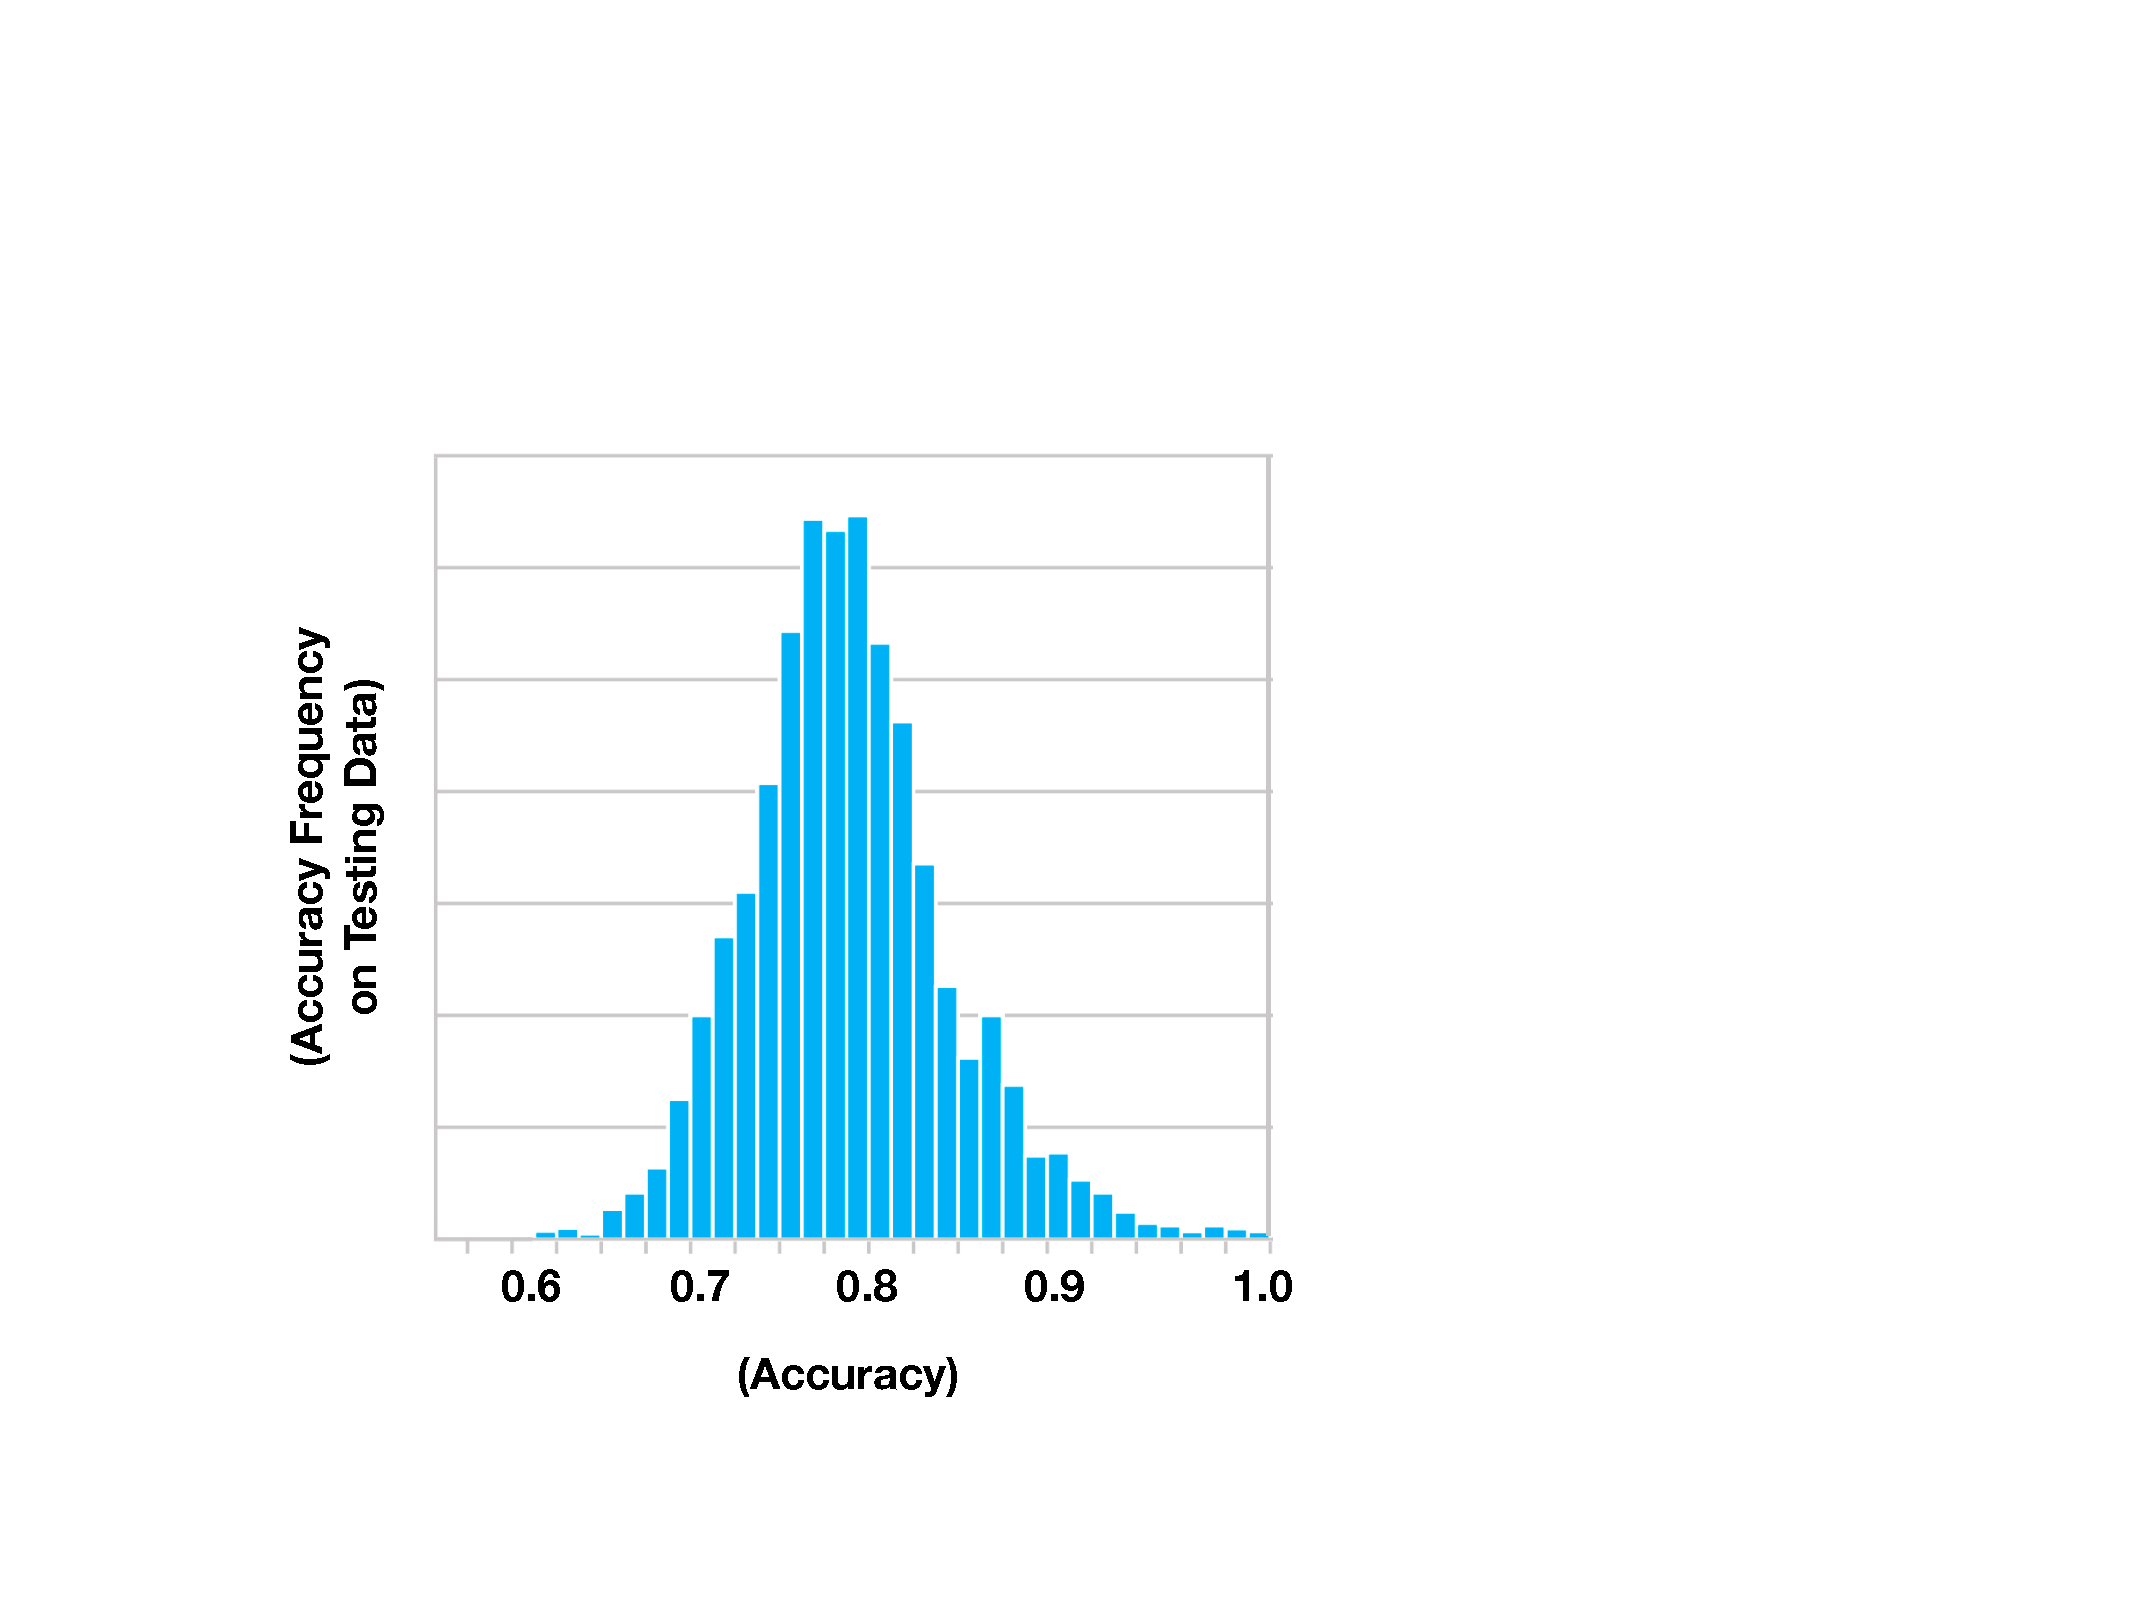
\includegraphics[width=0.4\textwidth]{figures/example_histogram.pdf}
        \caption{Example showing how your histograms should look like. The ``shape'' of the histograms you obtain may be different, of course.}
        \label{fig:sample_histogram}
    \end{figure} 
    %
    % YOUR RESPONSE HERE
    %

    
    
    \HIGHLIGHT{Q2.2 (12 Points)} In the second histogram, you should show the accuracy distribution when the algorithm was evaluated over \textit{testing data}. The horizontal axis should show different accuracy values, and the vertical axis should show the frequency with which that accuracy was observed while conducting these 100 experiments/training processes. You should also report the mean accuracy and its standard deviation.    
    %
    % YOUR RESPONSE HERE
    %
    

    \HIGHLIGHT{Q2.3 (12 Points)} Explain intuitively why each of these histograms look the way they do. Is there more variance in one of the histograms? If so, why do you think that is the case? Does one histogram show higher average accuracy than the other? If so, why do you think that is the case?
    %
    % YOUR RESPONSE HERE
    %

    
    \HIGHLIGHT{Q2.4 (8 Points)} By comparing the two histograms, would you say that the Decision Trees algorithm, when used in this dataset, is underfitting, overfitting, or performing reasonably well? Explain your reasoning.
    %
    % YOUR RESPONSE HERE
    %

    
    \HIGHLIGHT{Q2.5 (6 Points)} In class, we discussed how Decision Trees might be non-robust. Is it possible to experimentally confirm this property/tendency via these experiments, by analyzing the histograms you generated and their corresponding average accuracies and standard deviations? Explain your reasoning.
    %
    % YOUR RESPONSE HERE
    %
    
    \vspace{0.25in}
    \textbf{\HIGHLIGHT{Extra points (15 Points)} Repeat the experiment above but now using the Gini criterion for node splitting, instead of the Information Gain criterion.}
    %
    % YOUR RESPONSE HERE
    %
    
\end{enumerate}

\end{document}






